\documentclass[t]{beamer}
\usetheme[deutsch]{KIT}
\setbeamercovered{transparent}
\setbeamertemplate{navigation symbols}{}

\KITfoot{YUV.KA - Praxis der Softwareentwicklung WS 11/12}
\usepackage[utf8]{inputenc}
\usepackage{ngerman}
\usenavigationsymbols

\title{YUV.KA}
\subtitle{Abschlusspräsentation}
\author{Max Wagner $\cdot$ Patrick Gemander $\cdot$ Sebastian Ullrich $\cdot$ Michael Vollmer \\ Robert Hangu $\cdot$ Daniel Lebert}

\institute[ITEC]{Institut für Technische Informatik}

\TitleImage[trim = -20cm 0 0 0,height=\titleimageht]{logo.png}

\begin{document}

\begin{frame}
	\maketitle
\end{frame}

\begin{frame}
	\frametitle{Das Projekt}
	
	\begin{itemize}
		\item<+-> Ein Multimedia-Framework zur Evaluierung von Videoencodern
		\item<+-> Videos im YUV-Format einlesen und mit Syntheseoptionen verändern
		\item<+-> Videos mit Hife des Programms analysieren
	\end{itemize}
	\onslide<4>{$ \Longrightarrow $ Programm soll Entwicklern beim Testen ihrer Encoder helfen}
\end{frame}

\begin{frame}
	\frametitle{Die Lösung: YUV.KA}
	
	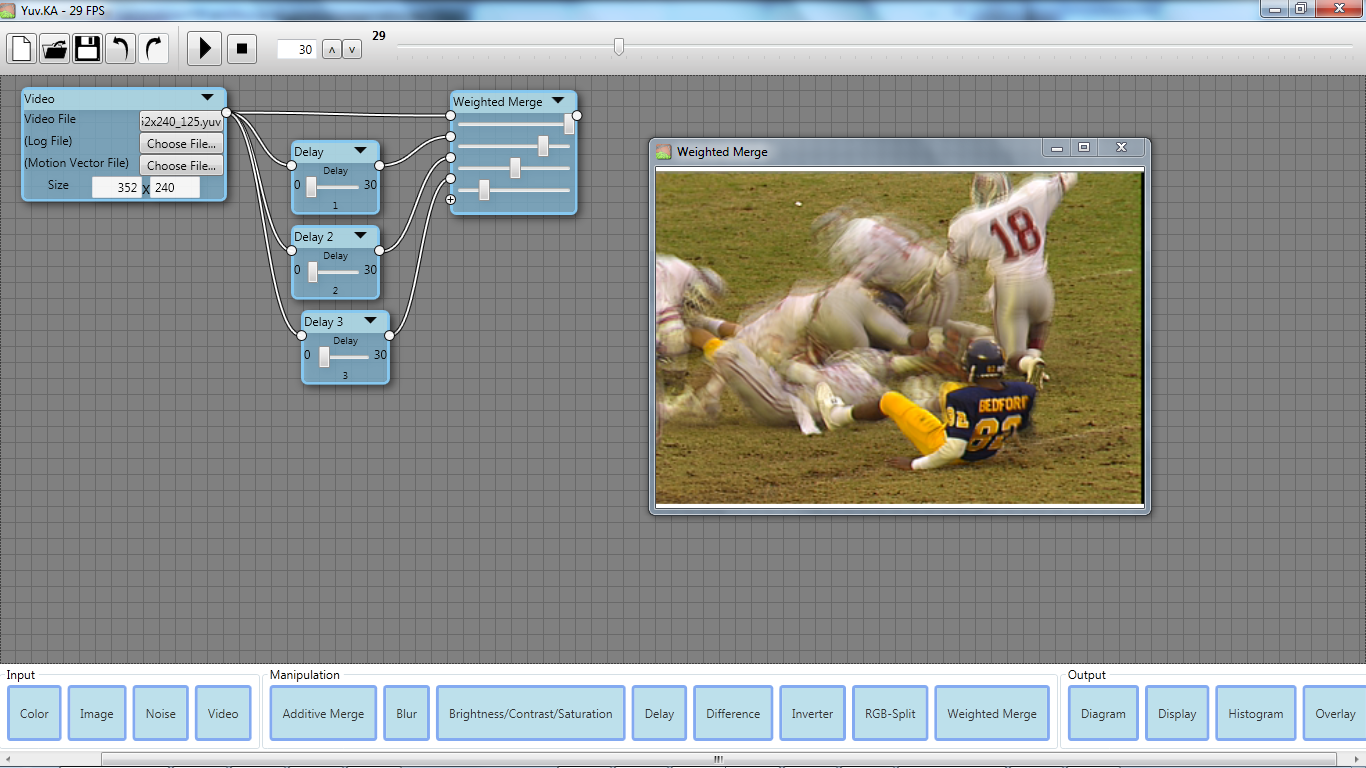
\includegraphics[width=11.3cm]{startup_screenshot.png}
\end{frame}

\begin{frame}
	\frametitle{Planung I}
	Videomanipulation ~\\
	\begin{itemize}
		\item<+-> Eingabe von Videos, Bildern, Farbe und Noise
		\item<+-> Farbkanäle trennen und Videos mergen
		\item<+-> Videos weichzeichnen
		\item<+-> Differenzvideos bilden
		\item<+-> Videoanalyse
	\end{itemize}
\end{frame}

\begin{frame}
	\frametitle{Planung II}
	
	Videoanalyse ~\\
	\begin{itemize}
		\item<+-> Histogramm
		\item<+-> Anzahl der Differenzen der Pixelfarben
		\item<+-> Anzahl der Artefakte und Artefaktoverlay
		\item<+-> Differenz der Encoderentscheidungen
	\end{itemize}
\end{frame}

\begin{frame}
	\frametitle{Planung III}
	
	Sonstige Features ~\\
	\begin{itemize}
		\item<+-> Erweiterbarkeit der Knotenmenge durch Plug-ins
		\item<+-> Parallelisiertes Rendering
	\end{itemize}
\end{frame}

\begin{frame}
	\frametitle{Entwurf I}
	
	Entwicklungsumgebung ~\\
	\begin{itemize}
		\item<+-> C\#
		\item<+-> WPF (\textbf{W}indows \textbf{P}resentation \textbf{F}oundation)
		\item<+-> Microsoft Visual Studio 2010
	\end{itemize}
\end{frame}

\begin{frame}
	\frametitle{Entwurf II}
	\noindent
	\begin{minipage}{3.5cm}
	    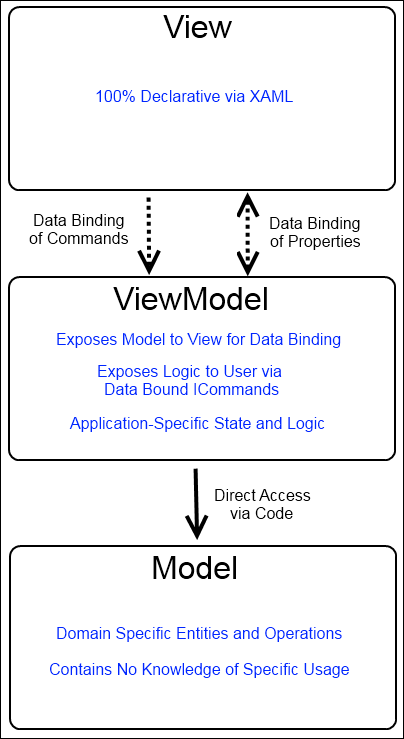
\includegraphics[width=3.5cm]{MVVM_thumb.png} ~\\
	    \textit{http://reedcopsey.com}
	\end{minipage}
	\hfill
	\begin{minipage}{8cm}
		Architektur - MVVM-Entwurfsmuster ~\\
	    \begin{itemize}	    
	    	\item<+-> Model-View-ViewModel
	        \item<+-> Eigens für WPF entwickeltes Entwurfsmuster
	        \item<+-> Erzielt Modularität und Testbarkeit durch vollständige Entkopplung von UI-Elementen und UI-Logik
	    \end{itemize}
	\end{minipage}
\end{frame}

\begin{frame}
	\frametitle{Implementierung I}

		
	
	% TODO: Statistiken
\end{frame}


\end{document}